    \vspace{-0.5cm}
\section{Vergleich der Elektrischen Maschinen}
    \renewcommand{\arraystretch}{0.6}
    \vspace{-0.5cm}
\begin{longtable}{| p{.30\textwidth} | p{.60\textwidth} |}
    \hline
    
    \textbf{Aufbau}&
    \tabbild[scale=0.5]{images/VergleichMotor}
    \\ \hline
    
    \textbf{Komplexität des Aufbaus}&
    \tabbild[scale=0.4]{images/VergleichMotorKomplex}
    \\ \hline
    
    \textbf{Kosten}&
    \tabbild[scale=0.4]{images/VergleichMotorKosten}
    \\ \hline
    
    \textbf{Wirkungsgrad}&
    \tabbild[scale=0.4]{images/VergleichMotorWirkungsgrad}
    \\ \hline
    
    \textbf{Anpassungsfähigkeit}&
    \tabbild[scale=0.4]{images/VergleichMotorAnpassung}
    \\ \hline
    
    \textbf{Anlaufstrom}&
    \tabbild[scale=0.4]{images/VergleichMotorAnlaufstrom}
    \\ \hline
    
    \textbf{Anlaufmoment}&
    \tabbild[scale=0.4]{images/VergleichMotorAnlaufmoment}
    \\ \hline
    
    \textbf{Drehzahlregelung}&
    \tabbild[scale=0.4]{images/VergleichMotorDrehzahl}
    \\ \hline
    
    \textbf{Anwendungsbereich}&
    \tabbild[scale=0.4]{images/VergleichMotorAnwendung}
    \\ \hline   
\end{longtable}   
\clearpage
\pagebreak
\subsection{Auswahl Flowchart} %TODO Grafik bi möglichkeit schärfer

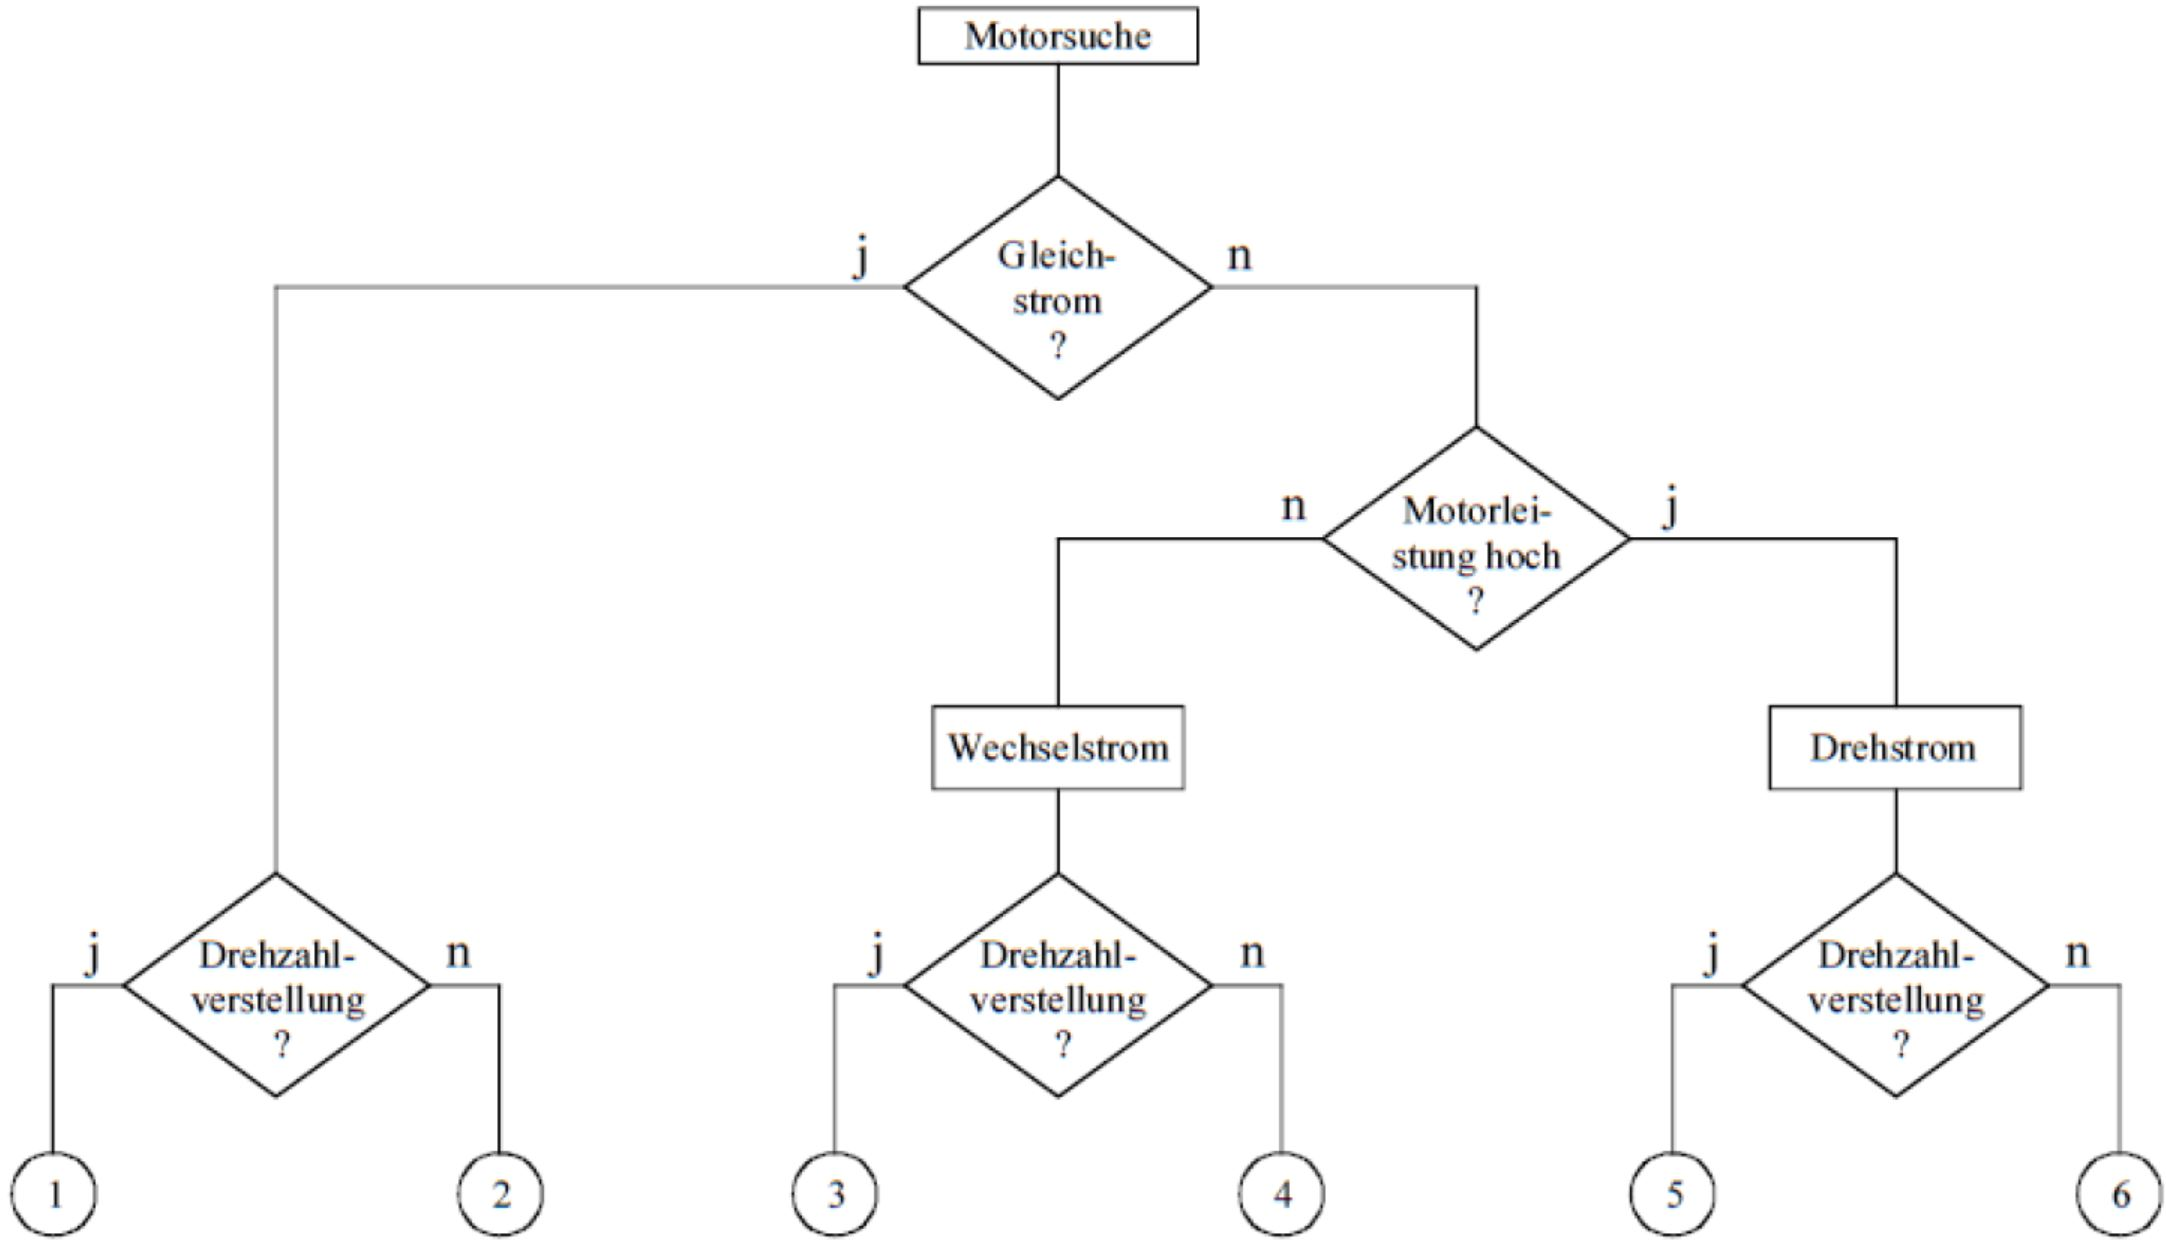
\includegraphics[scale=1]{images/Motorauswahl}
\\
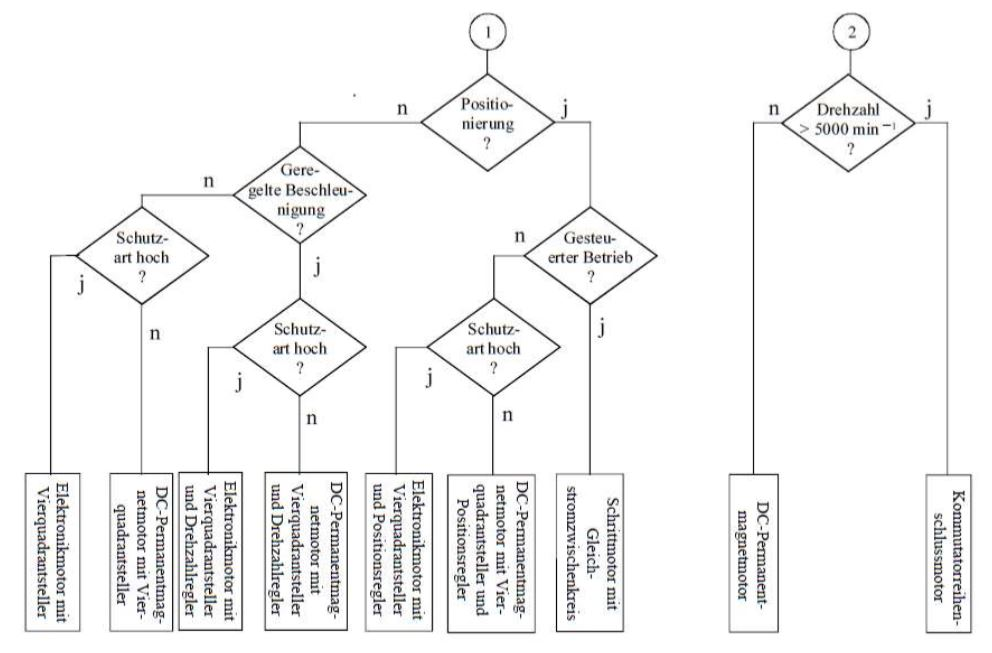
\includegraphics[scale=1]{images/Motorauswahl2}
\\
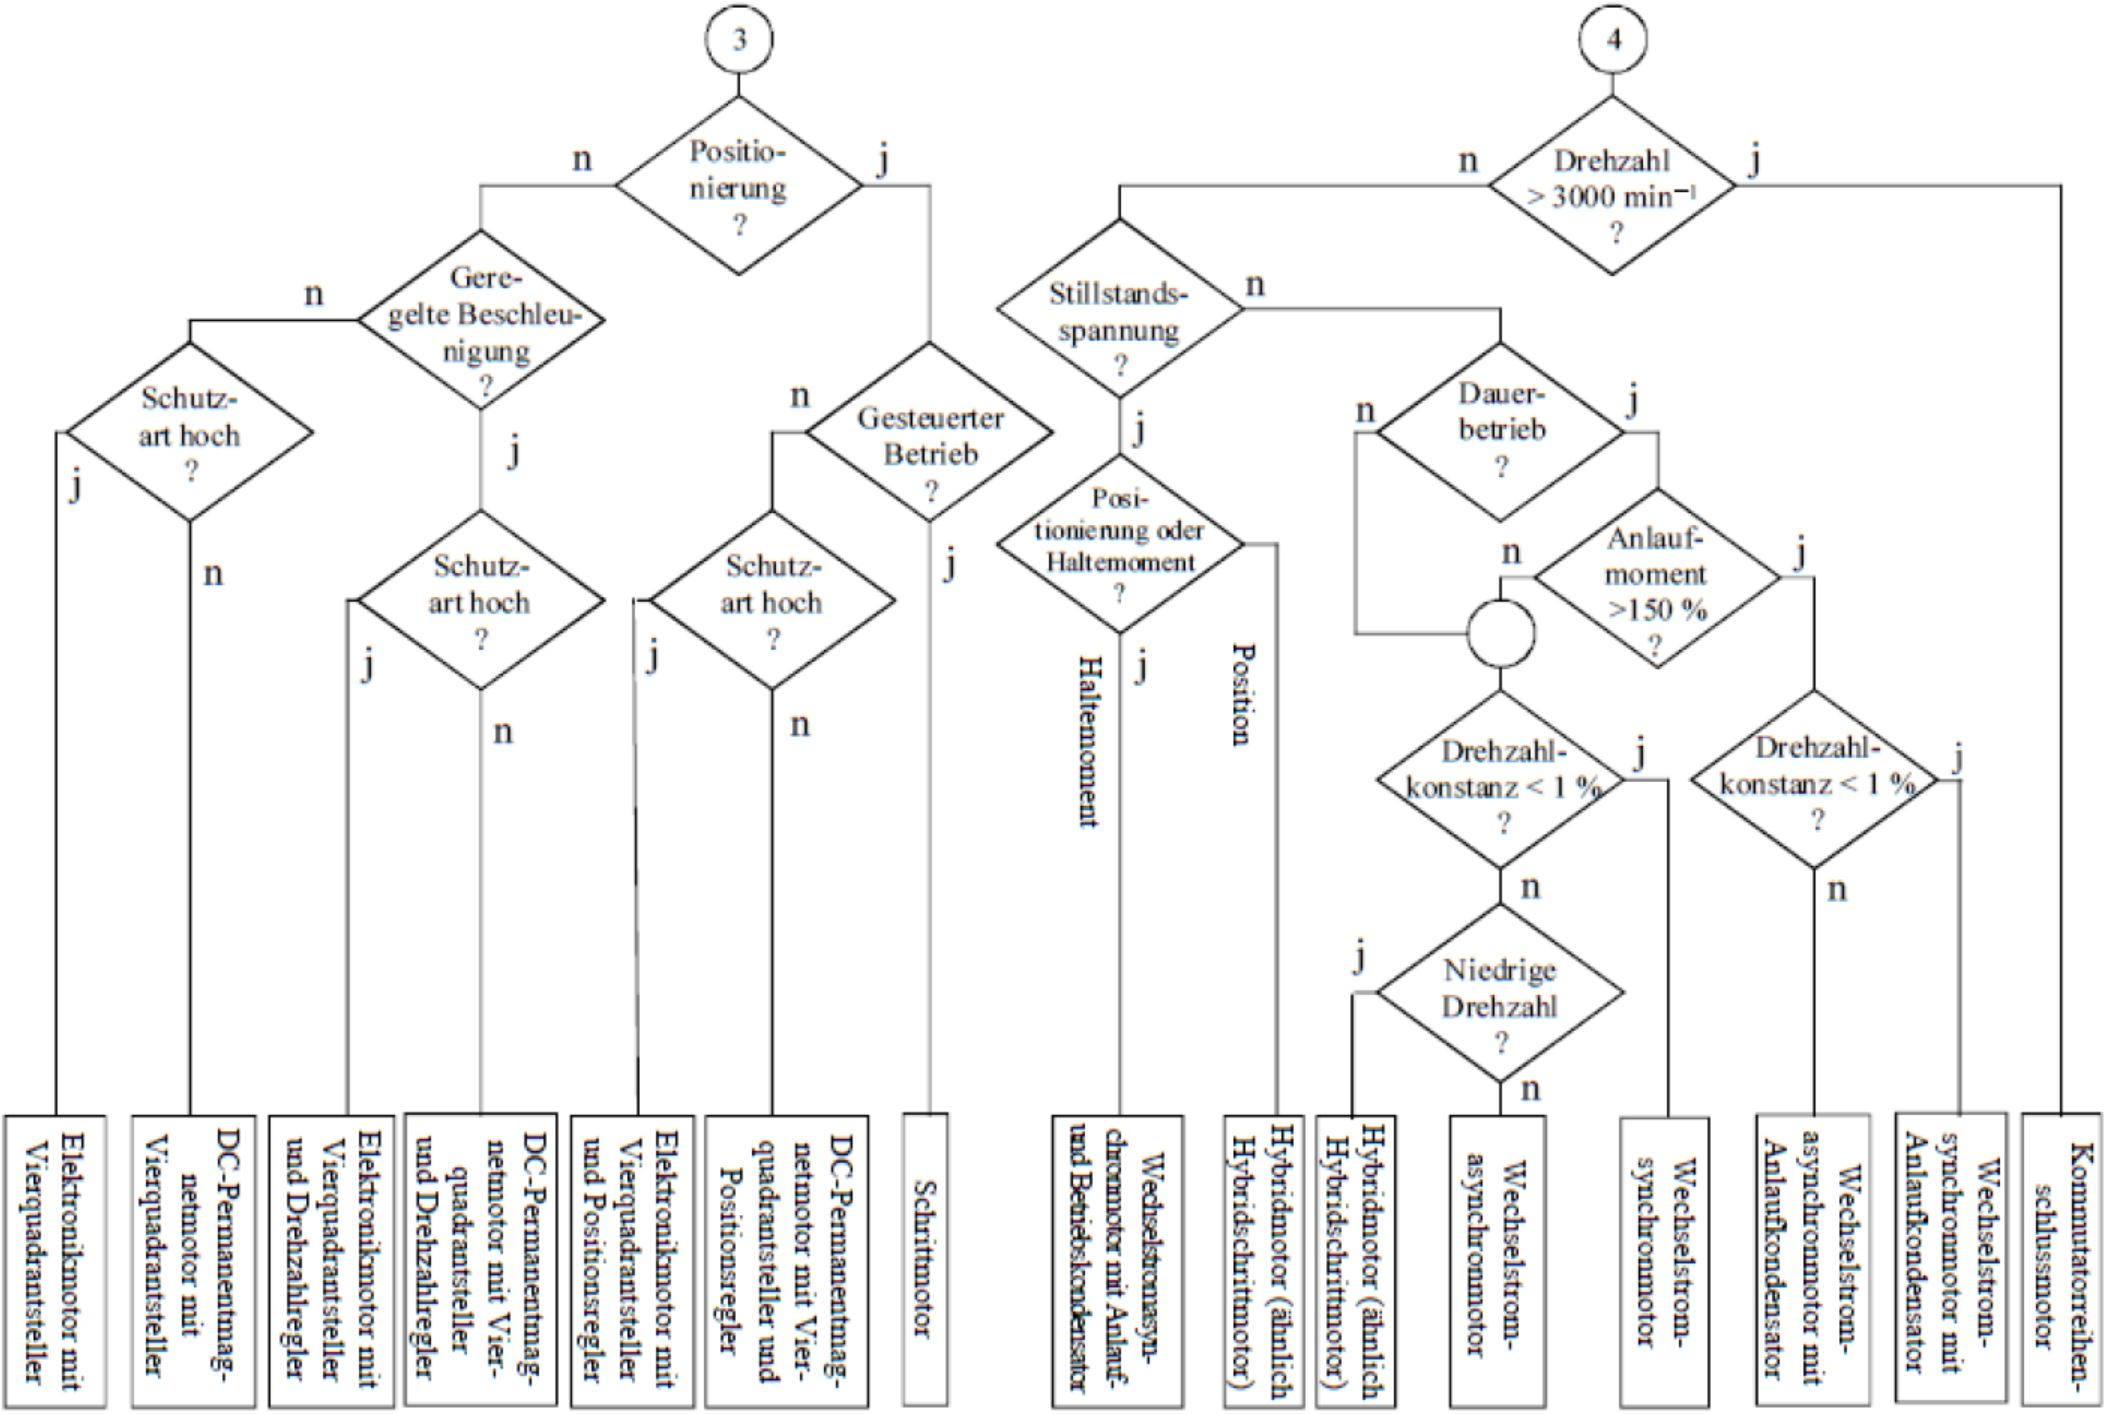
\includegraphics[scale=1]{images/Motorauswahl3}
\\
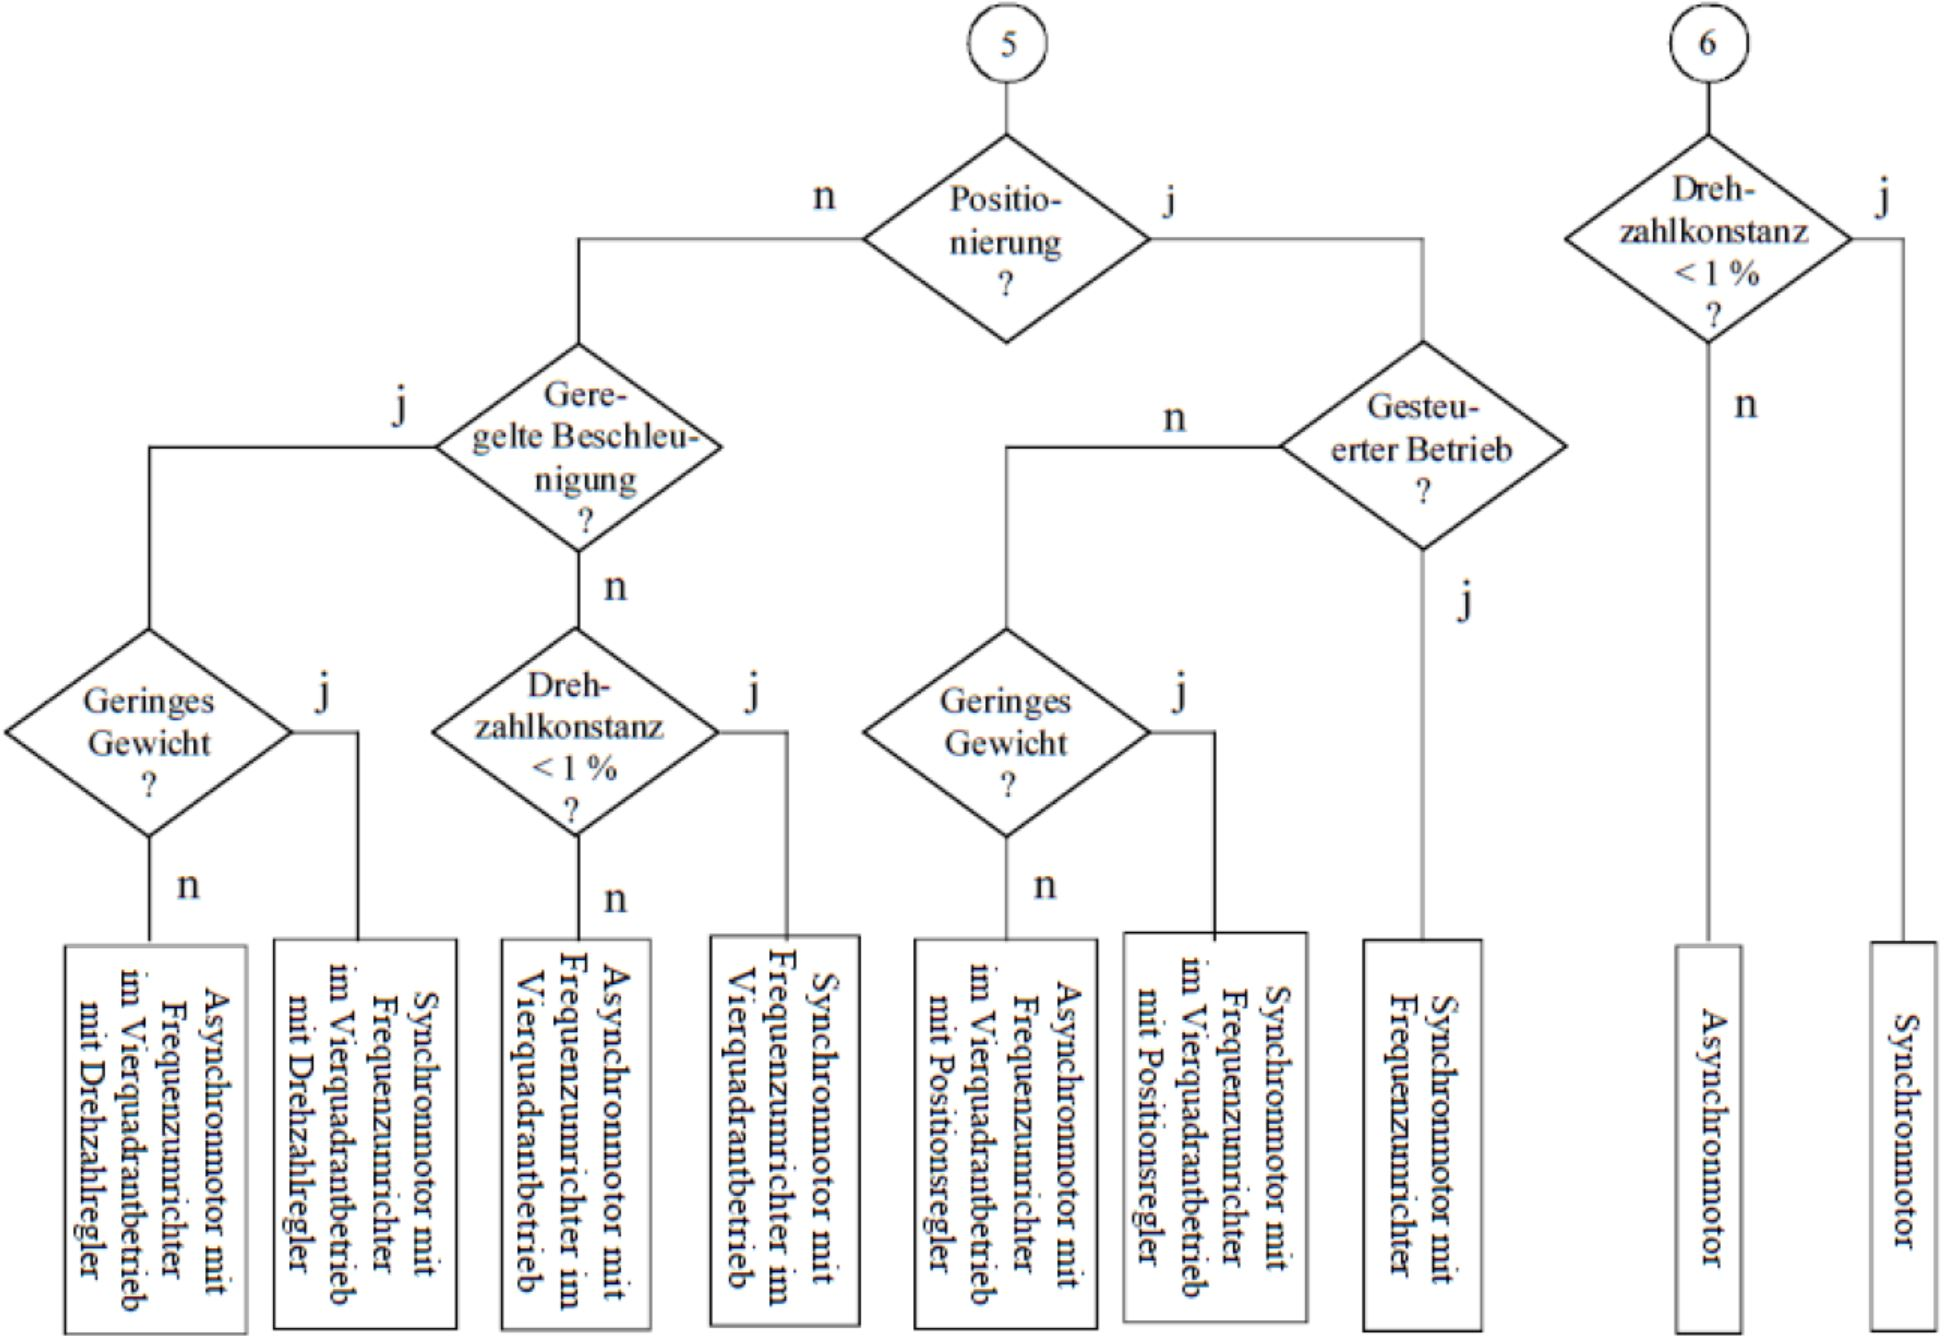
\includegraphics[scale=1]{images/Motorauswahl4}
\clearpage